\usetikzlibrary{arrows.meta, positioning, calc}

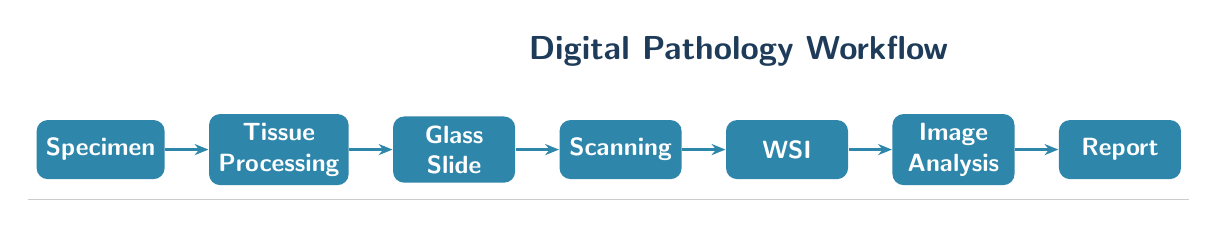
\begin{tikzpicture}[
    node distance = 0.55cm,
    every node/.style = {font=\small\sffamily},
    proc/.style = {
        rectangle,
        rounded corners=4pt,
        fill={rgb,255:red,46;green,134;blue,171},
        text=white,
        minimum width=1.55cm,
        minimum height=0.75cm,
        align=center,
        font=\small\sffamily\bfseries
    },
    arr/.style = {
        -{Stealth[length=5pt,width=4pt]},
        line width=0.8pt,
        color={rgb,255:red,46;green,134;blue,171}
    }
]

%% Title
\node[font=\large\sffamily\bfseries,
      text={rgb,255:red,30;green,60;blue,90}]
    (title) at (0,0) {Digital Pathology Workflow};

%% Nodes placed in a row below the title
\node[proc, below=0.55cm of title, xshift=-8.1cm] (specimen)  {Specimen};
\node[proc, right=0.55cm of specimen]              (tissue)    {Tissue\\Processing};
\node[proc, right=0.55cm of tissue]                (slide)     {Glass\\Slide};
\node[proc, right=0.55cm of slide]                 (scanning)  {Scanning};
\node[proc, right=0.55cm of scanning]              (wsi)       {WSI};
\node[proc, right=0.55cm of wsi]                   (analysis)  {Image\\Analysis};
\node[proc, right=0.55cm of analysis]              (report)    {Report};

%% Arrows
\draw[arr] (specimen) -- (tissue);
\draw[arr] (tissue)   -- (slide);
\draw[arr] (slide)    -- (scanning);
\draw[arr] (scanning) -- (wsi);
\draw[arr] (wsi)      -- (analysis);
\draw[arr] (analysis) -- (report);

%% Subtle baseline rule
\draw[line width=0.4pt, color=gray!40]
    ($(specimen.south west)+(-0.1,-0.25)$) --
    ($(report.south east)+(0.1,-0.25)$);

\end{tikzpicture}
